% Three-set Venn diagram for the proposal (compile with: pdflatex venn-tikz-example.tex).
% To paste into the proposal, copy everything between \begin{tikzpicture} and \end{tikzpicture}
% and add \usepackage{tikz} to the preamble (the proposal already loads TikZ for its Gantt charts).
\documentclass[tikz,border=6pt]{standalone}
\begin{document}
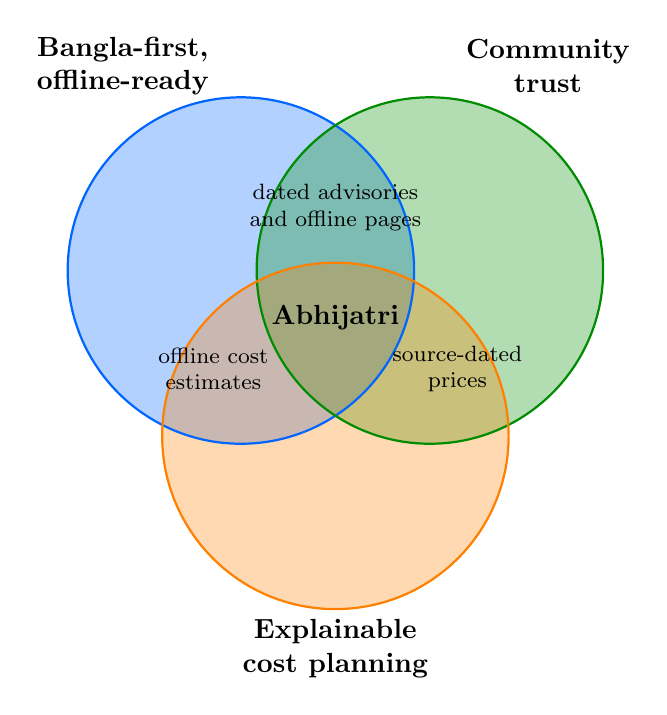
\begin{tikzpicture}[font=\sffamily\small]
  \def\r{2.2}
  \colorlet{cA}{blue!60!cyan}
  \colorlet{cB}{green!55!black}
  \colorlet{cC}{orange}
  % 30 percent opacity lets the overlaps show through
  \fill[cA,opacity=.30] (-1.2, 0.7) circle (\r);
  \fill[cB,opacity=.30] ( 1.2, 0.7) circle (\r);
  \fill[cC,opacity=.30] ( 0  ,-1.4) circle (\r);
  \draw[cA,thick] (-1.2, 0.7) circle (\r);
  \draw[cB,thick] ( 1.2, 0.7) circle (\r);
  \draw[cC,thick] ( 0  ,-1.4) circle (\r);
  % set names
  \node[font=\bfseries,align=center] at (-2.7, 3.3) {Bangla-first,\\offline-ready};
  \node[font=\bfseries,align=center] at ( 2.7, 3.3) {Community\\trust};
  \node[font=\bfseries,align=center] at ( 0  ,-4.1) {Explainable\\cost planning};
  % overlaps (what each pair gives)
  \node[align=center,font=\footnotesize] at ( 0  , 1.5) {dated advisories\\and offline pages};
  \node[align=center,font=\footnotesize] at (-1.55,-0.55) {offline cost\\estimates};
  \node[align=center,font=\footnotesize] at ( 1.55,-0.55) {source-dated\\prices};
  \node[align=center,font=\bfseries] at (0, 0.1) {Abhijatri};
\end{tikzpicture}
\end{document}
